
\documentclass[letter,12pt]{article} 

\usepackage[top = 5cm, bottom = 2.5cm, left = 2.5cm, right = 2.5cm]{geometry}  
\usepackage[T1]{fontenc}
\usepackage[utf8]{inputenc}
\usepackage[spanish,es-tabla]{babel}
\spanishdecimal{.}
\usepackage{multirow} 
\usepackage{booktabs} 
\usepackage{graphicx} 
\usepackage{epstopdf}
\usepackage{setspace}
\setlength{\parindent}{0in}
\usepackage{float}
\usepackage{fancyhdr}
\usepackage{amsmath,mathtools}
\usepackage{amsfonts}
\usepackage{amssymb}
\usepackage{xcolor}
\usepackage{pdfpages}
\usepackage{apacite}
\usepackage{subfig}


\pagestyle{fancy} 

\fancyhf{} 

\lhead{\footnotesize  Propuesta/Boceto de proyecto} 	
\rhead{\footnotesize Gallardo Tinoco} 

\cfoot{\footnotesize \thepage} 	


\begin{document}
\begin{titlepage}
	
	\begin{center}
		\vspace*{-1in}

		
		UNIVERSIDAD NACIONAL AUTONOMA DE MEXICO\\
		\vspace*{0.15in}
		FACULTAD DE INGENIERÍA \\
		\vspace*{0.15in}
		INGENIERÍA EN COMPUTACIÓN \\
		\vspace*{0.6in}
		\begin{large}
			Laboratorio de Computación Grafica E Interacción Humano-Computadoras\\
		\end{large}
		\vspace*{0.1in}
		\rule{160mm}{0.1mm}\\
		\vspace*{0.1in}
		\begin{large}
			Grupo: 11\\
			Semestre 2021-2\\
		\end{large}
		\vspace*{0.2in}
		\begin{Large}
			\textbf{Propuesta/Boceto de proyecto} \\
		\end{Large}
		\vspace*{0.3in}
		\rule{80mm}{0.1mm}\\
		\vspace*{0.1in}
		\begin{large}
			418046595 \\
			andrwe713@gmail.com \\
			Gallardo Tinoco Andrés Amadeus\\
		\end{large}
	\end{center}
	
\end{titlepage}
\newpage
Se planea desarrollar una cocina de un restaurante.
	\begin{figure}[H]
		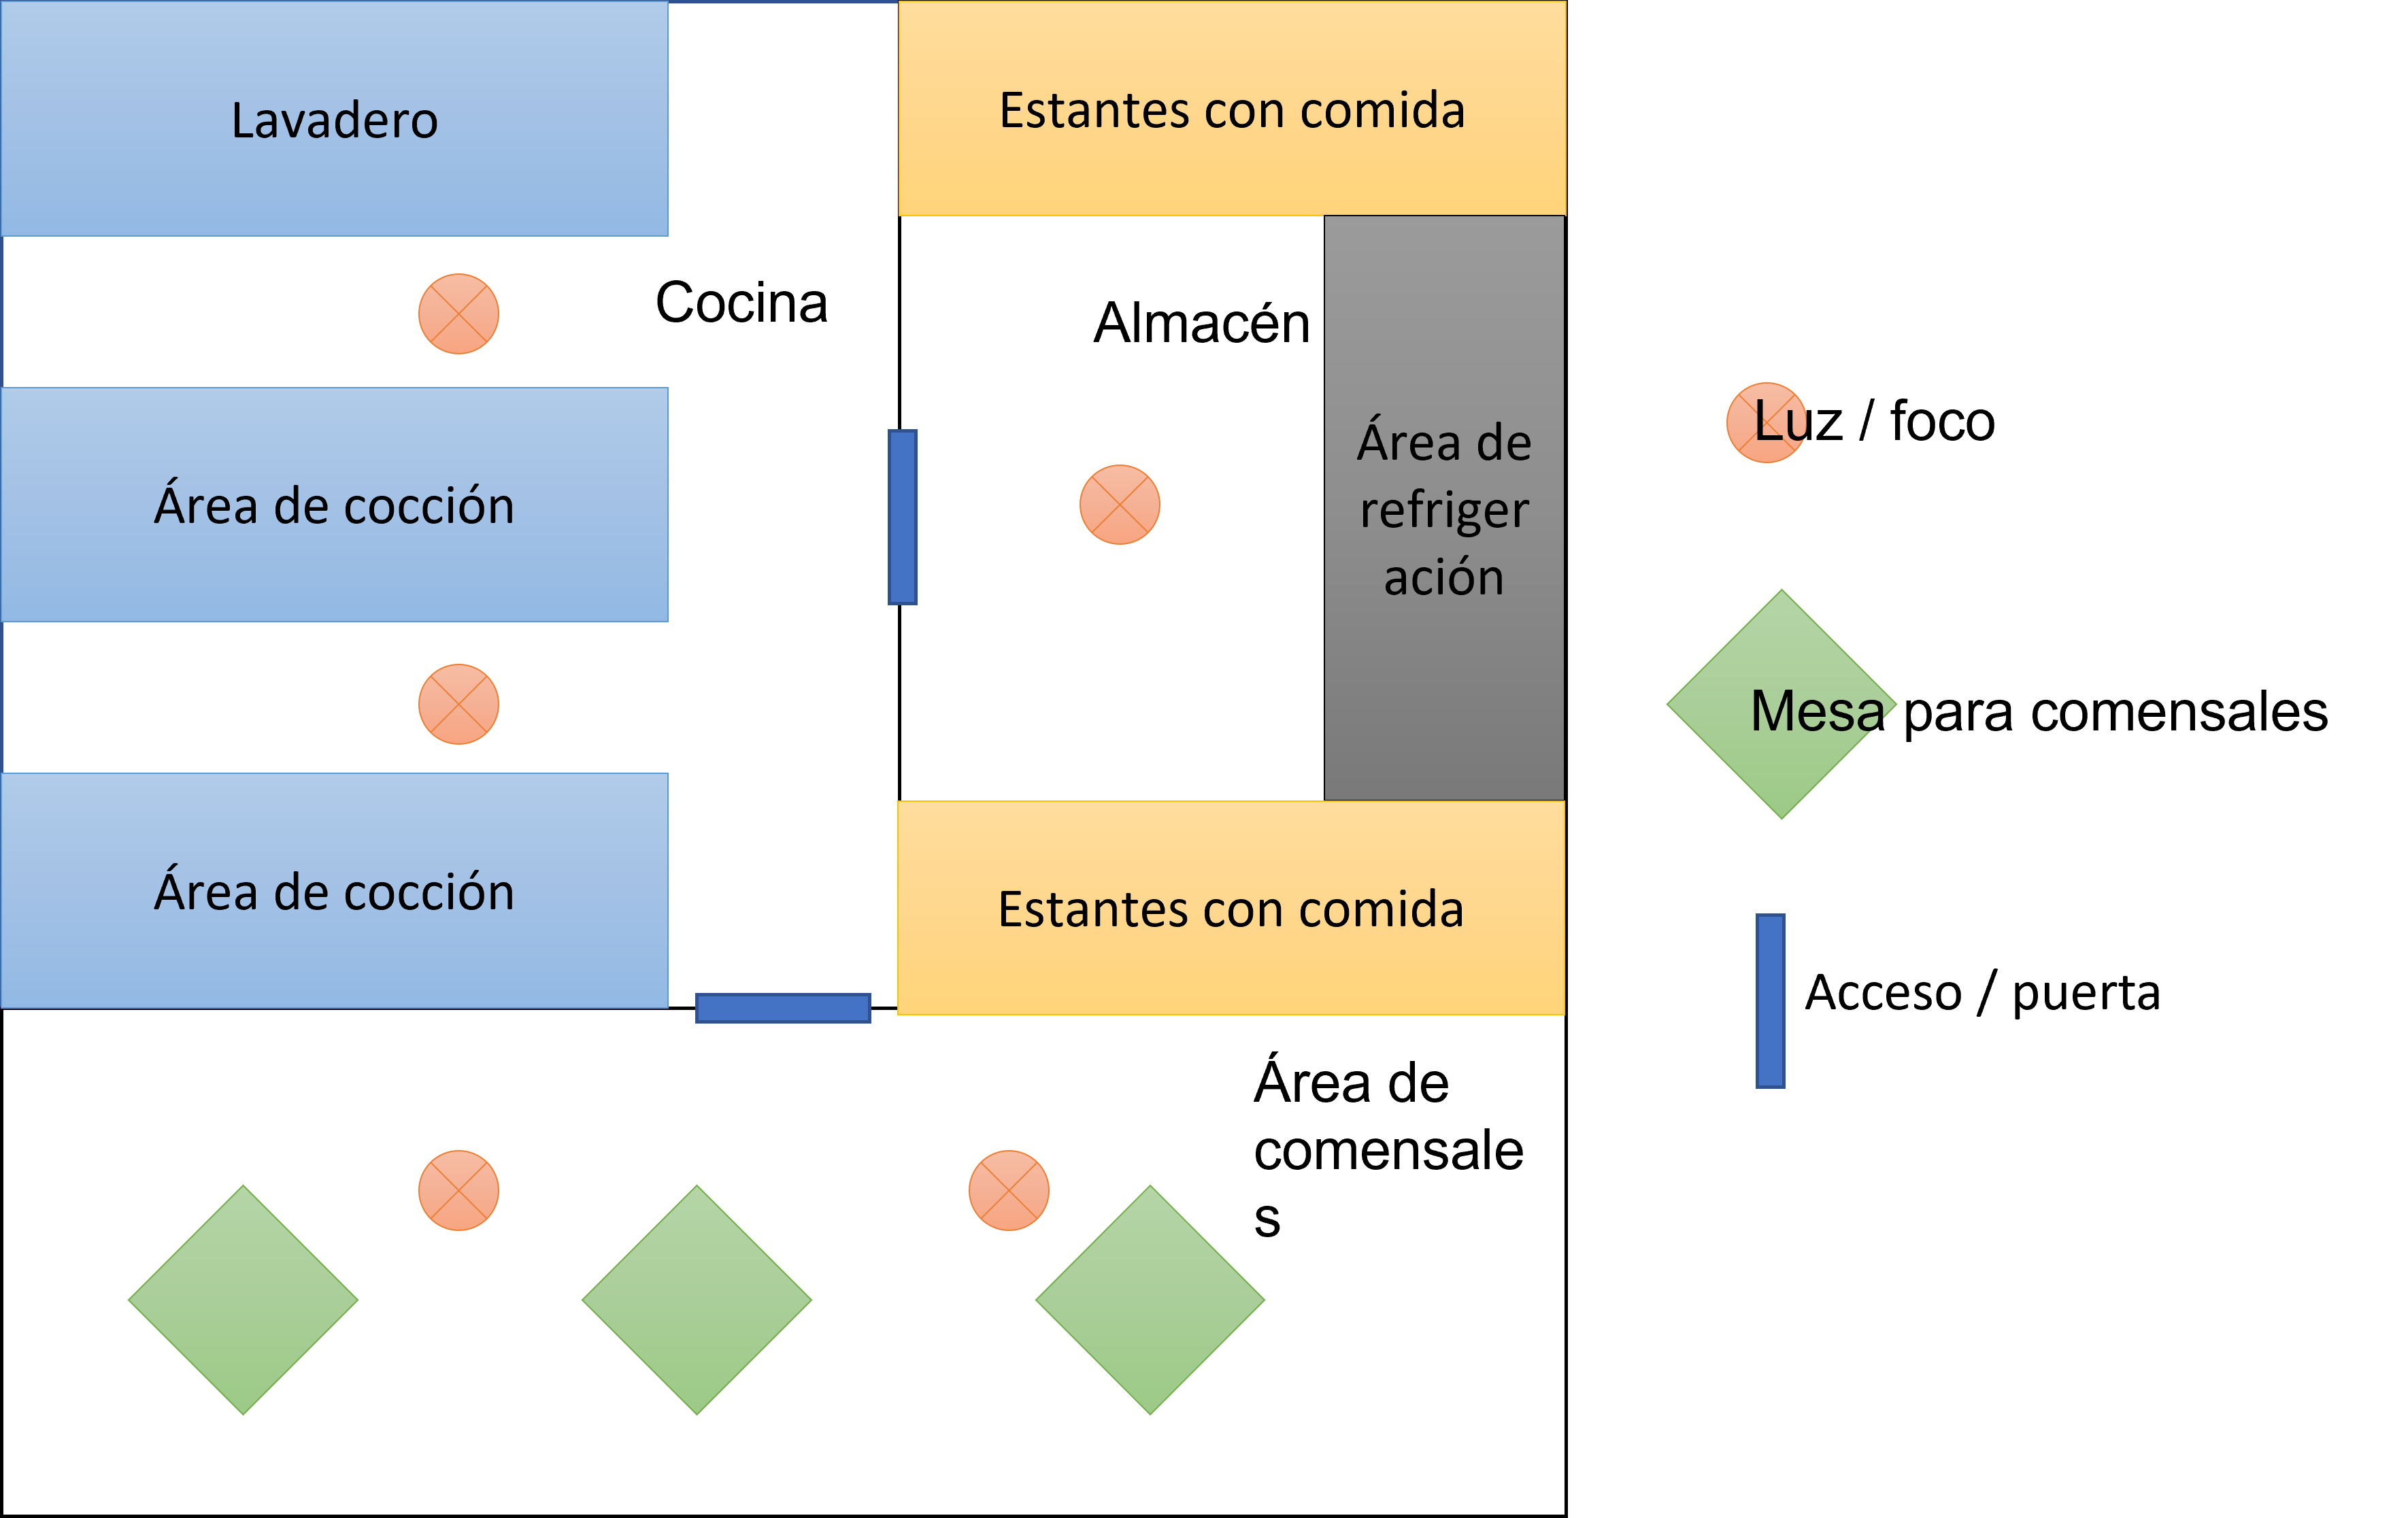
\includegraphics[scale=0.6]{img1}
		\centering
		\caption{Mapeado final propuesto}
	\end{figure}
Este será un entorno cerrado, con la iluminación básica de una cocina de un restaurante.\\
Como animaciones básicas estas podrían ser:
\begin{itemize}
\item Animación sobre puertas de alacenas o gabinetes.
\item Animación sobre alguna estufa, planteando cocinar algo.
\item Animación sobre platos lavándose, o fregadero funcionando.
\item Animación sobre mesa describiendo alguna receta preparándose (Amasar un poco de masa, revolver contenido de un bol)
\item Animación sobre horno saliendo un pan o una pizza.
\item Animación de una jarra de agua sirviendo un sobre un vaso.

\end{itemize}
Estas son algunas ideas de las animaciones que se podría realizar, todas las animaciones incluyen un sonido que sera el representativo, por ejemplo al momento de abrir una puerta tendra el sonido de abrir una puerta, sin embargo, aún no se tienen las animaciones finales de manera especifica cada una.\\

\section{Cocina}
Dentro de esta area, el piso sera de azulejos, con paredes blancas y luces blancas.

\subsection{Lavadero}
Se planea modelar un lavadero, es decir una mesa de metal con un lavadero, tambien en esto modelar trastes sucios como limpios secandose a un costado del lavadero.

\subsection{Área de cocción}
Nuevamente son mesas de metal, con sus respectivas parrillas o hornos, y algunas ollas o sartenes con comida, de igual forma pueden llevar algunos elementos como botes de condimentos, botellas, servilletas, utencilios, etc.
Dentro de las areas de coccion tambien se llevaran a cabo animaciones como antes se habian propuesto.

\section{Almacen}
Sera un area de paredes grises, con piso de azulejo igual que la cocina, habra elementos en el suelo, como cajas vacias, unas escaleras, costales de comidad, etc.

\subsection{Estantes con comida}
Seran estantes de madera, con comida en ellos, cajas de verduras y frutas, cajas de latas, bolsas de comidad como sopas, semillas, etc. tambien habra productos sueltos.

\subsection{Área de refrigeración}
Seran refrigeradores, que contendran comidad, carne, queso, etc, la puerta se podra abrir y cerrar.

\section{Área de comensales}
Sera un area de piso de azulejo diferente al de la cocina, con elementos como macetas con plantas, etc.

\subsection{Mesa para comensales}
Seran mesas de una forma poligonal, con su respectivo numero de sillas, tendra arriba elementos como saleros, servilletas, platos, vasos, jarras de agua, etc.

\section{personaje}
Como último punto se planea desarrollar como avatar a un chef, este no es de ninguna compañía, será creado de manera generalizada, es decir un personaje humanoide con una filipina, zapatos y su característico gorro de chef.

	\begin{figure}[H]
		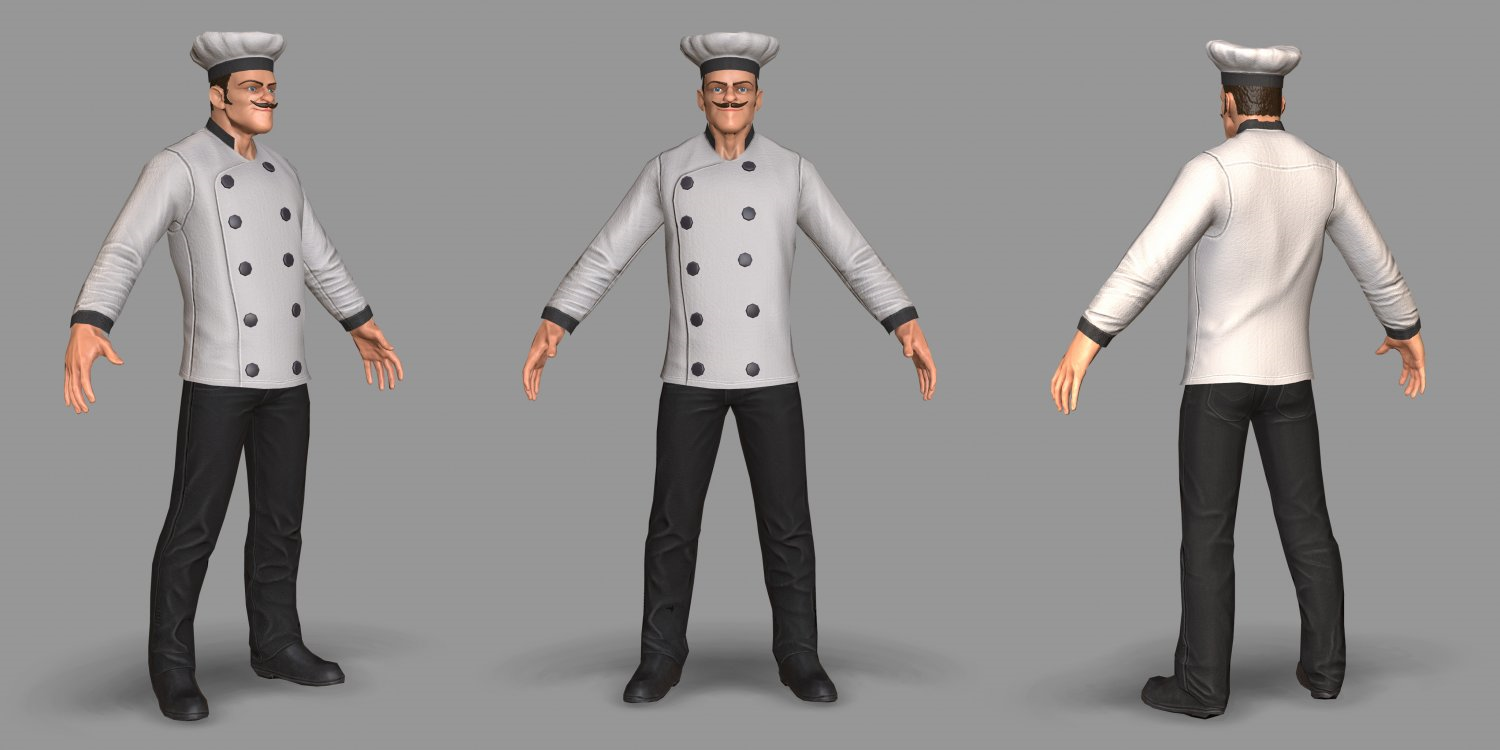
\includegraphics[scale=0.25]{img2}
		\centering
		\caption{No es una idea final, solo es un apoyo para hacer referencia al modelo que se plantea realizar}
	\end{figure}

\end{document}

	\begin{figure}[H]
		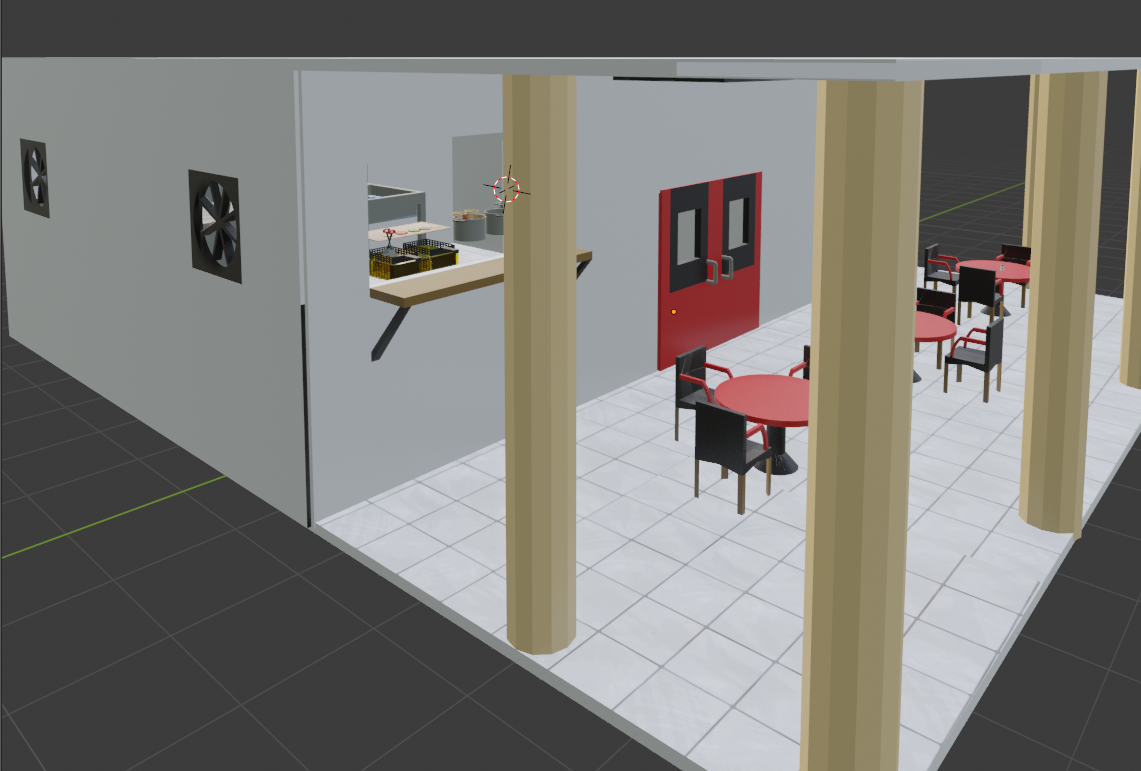
\includegraphics[scale=0.5]{img/img1}
		\centering
		\caption{Diagrama simulado en Multisim}
	\end{figure}

	\begin{figure}[H]
	 \centering
	  \subfloat[Osciloscopio]{
	    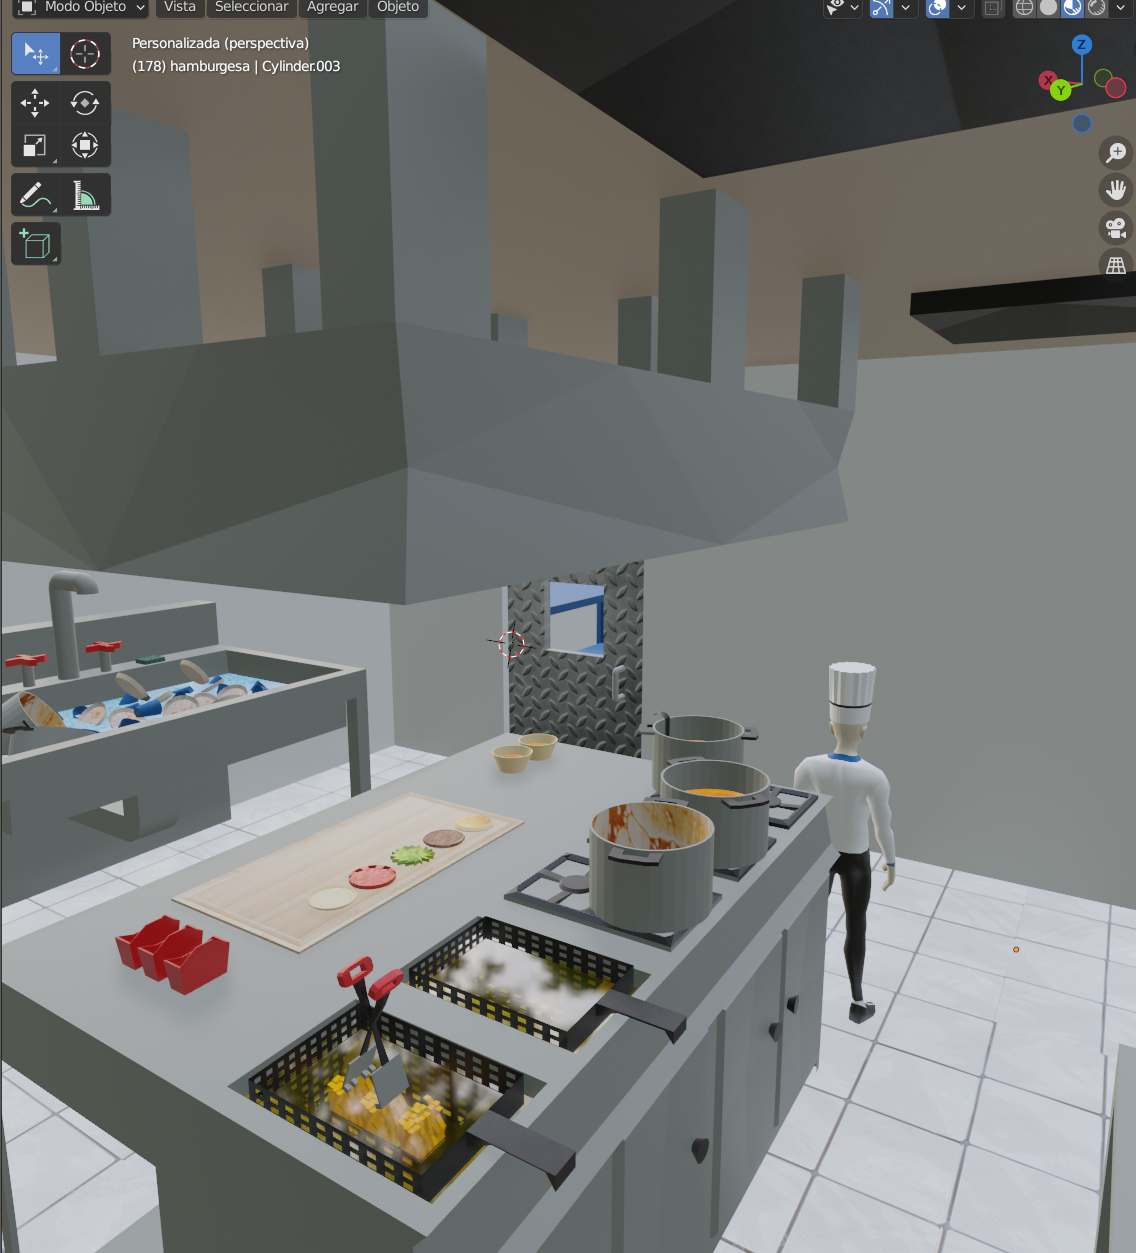
\includegraphics[width=0.45\textwidth]{img/img2}}
	  \subfloat[Analizador de espectro]{
	    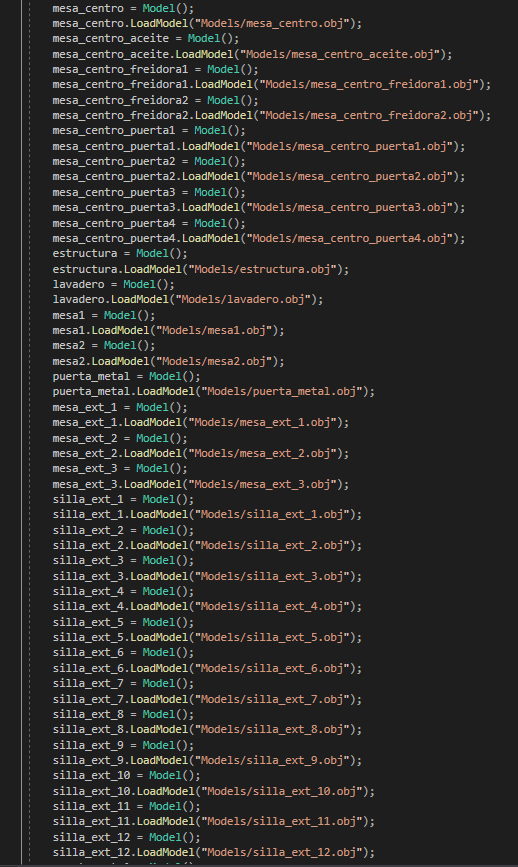
\includegraphics[width=0.45\textwidth]{img/img3}}
	 \caption{Salidas obtenidas}
	\end{figure}
